\cleardoublepage
\phantomsection
\addcontentsline{toc}{chapter}{Introduction}
\chapter*{Introduction\markboth{INTRODUCTION}{}}
This report contains the designs that led to the final tube notching machine. An overview of the purpose, usage, and requirements for the machine are given. The Notchmatic and its components are described in detail. Design calculations are given. A full bill of materials and cost report are provide. Part and assembly drawings are given as well. All datasheets for off-the-shelf parts are given. For usage, installation, maintenance, and safety information, please wait until the end of the spring semester. 

All of the files (CAD, reports, etc.) related to the machine can be downloaded from our git repository. 

\begin{figure}[htp]
    \centering
    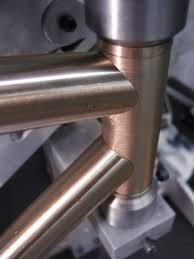
\includegraphics[width=0.4\textwidth]{./fall-report pictures/Chapter1-Basics/notched-tube}
    \caption{A welded notched tube.}
    \label{fig:notched-tube}
\end{figure}

